\section{Ablations and Recovery Analysis}
\label{sec:analysis}

We test whether the gains require compiled Cards, Registry validation, grounded
arguments, and selective admission.

\subsection*{Ablation Studies}

Tables~\ref{tab:compiled-selection} and
\ref{tab:controller-gate-ablation} evaluate full test trajectories;
Table~\ref{tab:card-structure-ablation} uses same-state forks.

\textbf{Prompts and Registry validation.}
Table~\ref{tab:compiled-selection} replaces Cards with generic reconsideration
prompts at Functional Loop or exact-repeat triggers. Neither improves on Raw.
The unvalidated Registry does improve task outcomes, but intervenes more often
and incurs more observed losses. The nine-Card validated Registry gives the
best Pass@1 and UX with one observed loss, showing that mining finds useful
actions while validation makes their deployment more selective.

\begin{table*}[!t]
\centering
\scriptsize
\renewcommand{\arraystretch}{0.9}
\setlength{\tabcolsep}{2.5pt}
\begin{tabular*}{\textwidth}{@{\extracolsep{\fill}}lrrrrrrrrrr@{}}
\toprule
Variant & Pass@1 & $\Delta$ & Pass$^5$ & $\Delta$ & UX & $\Delta$
& Triggered & W/T/L & Obs. Loss & Obs. Net \\
\midrule
Raw & 56.9 & -- & 30.0 & -- & 3.72 & -- & 0/750 & -- & -- & -- \\
Functional Loop + Generic Prompt & 55.5 & $-1.4$ & 28.0 & $-2.0$ & 3.65 & $-0.07$
& 51/750 & 0/50/1 & 2.0\% & $-2.0$\% \\
Exact Repeat + Generic Prompt & 56.7 & $-0.3$ & 30.7 & $+0.7$ & 3.69 & $-0.04$
& 102/750 & 6/87/9 & 8.8\% & $-2.9$\% \\
Unvalidated (All Cards) & 58.5 & $+1.6$ & \textbf{36.0} & $+6.0$ & 3.74 & $+0.02$
& 169/750 & 28/126/15 & 8.9\% & $+7.7$\% \\
Validated (9 Cards) & \textbf{59.5} & \textbf{$+2.6$} & 34.0 & $+4.0$ & \textbf{3.75}
& \textbf{$+0.03$} & 45/750 & 13/31/1 & 2.2\% & $+26.7$\% \\
\bottomrule
\end{tabular*}
\setlength{\tabcolsep}{6pt}
\renewcommand{\arraystretch}{1.0}
\caption{Recovery and Registry ablation on STATE-Bench with
DeepSeek-v4-Flash. Deltas are relative to Raw; triggered diagnostics use
matched task-runs. Each variant contains 750 test trajectories.}
\label{tab:compiled-selection}
\end{table*}

\textbf{Card content.}
On 49 held-out same-state forks, Full Cards solve 24 states versus 9 without
intervention. Operator-Only provides no gain, and removing argument grounding
reaches 16. The effect therefore depends on executable arguments and
constraints, not an operator label alone.

\begin{table}[t]
\centering
\scriptsize
\setlength{\tabcolsep}{1.5pt}
\begin{tabular*}{\columnwidth}{@{\extracolsep{\fill}}lrrrr@{}}
\toprule
Recovery branch & Success & $\Delta$ & W/T/L & Harm \\
\midrule
No Intervention & 9/49 (18.4\%) & -- & -- & -- \\
Full Card & \textbf{24/49 (49.0\%)} & \textbf{+30.6} & 16/32/1 & 2.0\% \\
Operator-Only & 9/49 (18.4\%) & 0.0 & 0/49/0 & 0.0\% \\
No Arg. Grounding & 16/49 (32.7\%) & +14.3 & 7/42/0 & 0.0\% \\
\bottomrule
\end{tabular*}
\caption{Same-state Card-content ablation on 49 held-out pre-action states.
Diagnostics and $\Delta$ are relative to No Intervention.}
\label{tab:card-structure-ablation}
\end{table}

\textbf{Admission gate.}
Removing proposed-action and recent-progress guards raises interventions from
45 to 50 but lowers all three task measures and doubles observed harm. Broader
admission therefore does not improve this rerun.

\begin{table}[t]
\centering
\scriptsize
\setlength{\tabcolsep}{2pt}
\begin{tabular*}{\columnwidth}{@{\extracolsep{\fill}}lrrrrrr@{}}
\toprule
Controller & Pass@1 & Pass$^5$ & UX & Triggered & W/T/L & Harm \\
\midrule
Full & \textbf{59.5} & \textbf{34.0} & \textbf{3.75} & 45/750 & 13/31/1 & 2.2\% \\
No-Guard & 58.5 & 32.0 & 3.71 & 50/750 & 12/36/2 & 4.0\% \\
\bottomrule
\end{tabular*}
\caption{Controller-gate ablation on an independent 750-trajectory rerun.
Triggered W/T/L and harm are descriptive diagnostics against Raw.}
\label{tab:controller-gate-ablation}
\end{table}

\textbf{Summary.}
Together, the ablations locate the improvement in the full recovery pipeline:
generic prompts do not reliably repair stalled states, unvalidated Cards show
that the mined actions are useful but too exposed, operator-only Cards lose the
effect, and wider admission increases risk. PERSIST-ACE works best when the
controller combines a validated Registry, grounded Card arguments, and
selective admission before replacing the base model's action.

\subsection*{Recovery Behavior on STATE-Bench}

The following analysis fixes STATE-Bench and varies the base model. It focuses
on triggered and Functional Loop-exposed trajectories rather than
averaging over the many runs on which PERSIST-ACE correctly abstains.

\begin{figure}[!t]
\centering
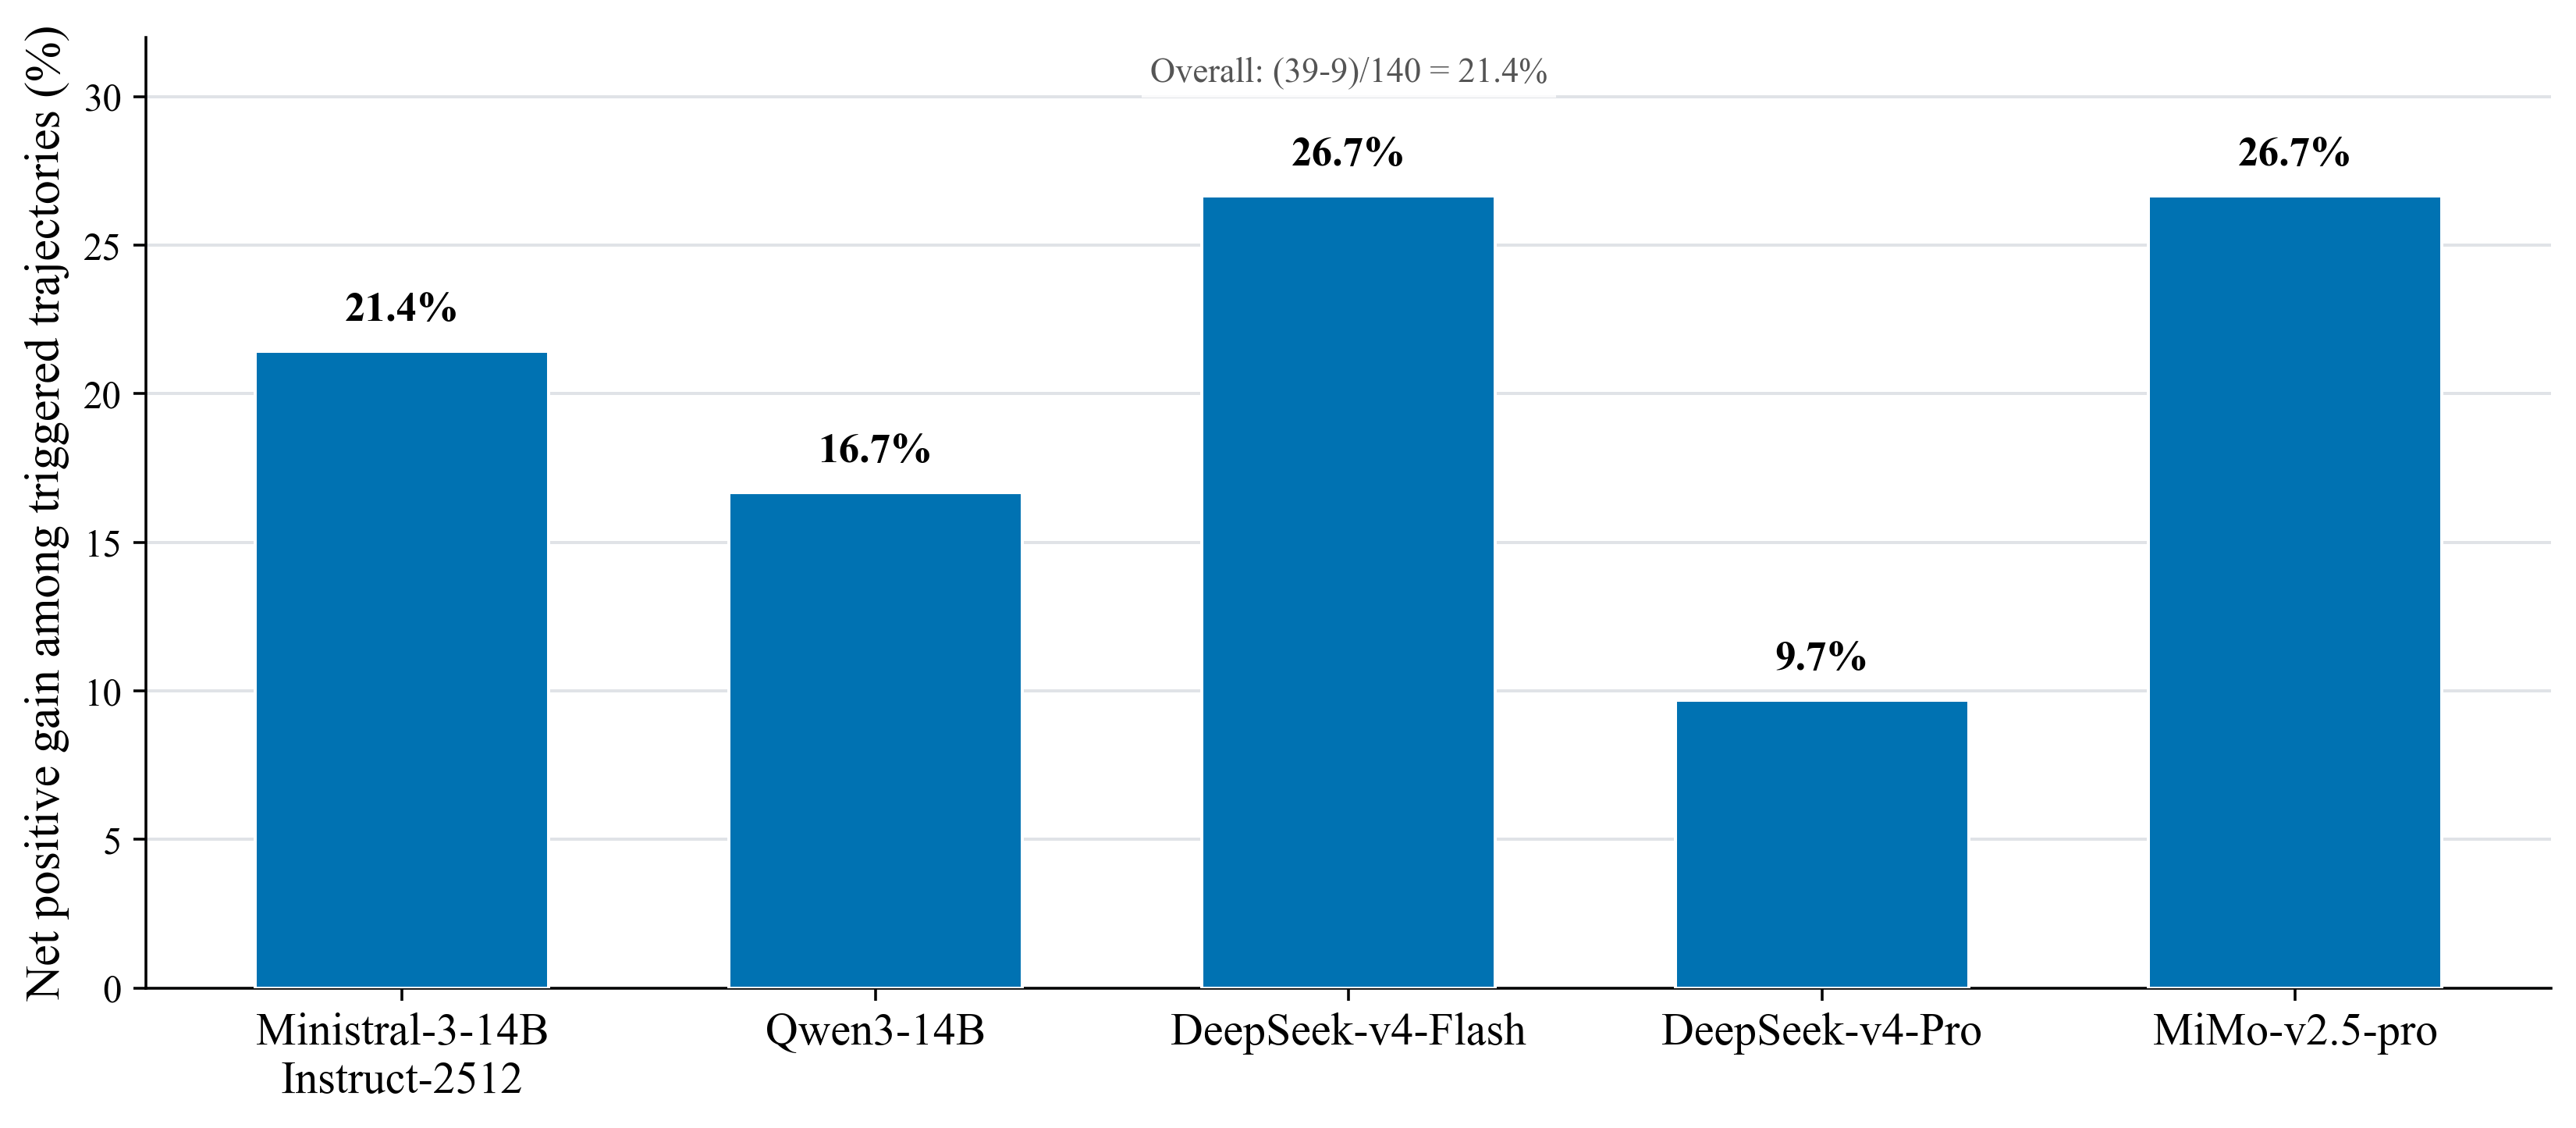
\includegraphics[width=\columnwidth]{figures/fig_statebench_triggered_failure_recovery.png}
\caption{Net outcome gain among triggered STATE-Bench trajectories. Each bar
reports $(W-L)/N_{\mathrm{triggered}}$ from paired Raw and PERSIST-ACE runs.
The overall margin is $(39-9)/140=21.4\%$.}
\label{fig:triggered-failure-recovery}
\end{figure}

\textbf{Triggered trajectories.}
Figure~\ref{fig:triggered-failure-recovery} shows a positive net outcome margin
for every model. Across 140 triggered trajectories, PERSIST-ACE produces 39
wins and 9 losses, yielding 30 net gains. The magnitude varies with the base
model, but the consistently positive direction indicates that the frozen
Registry transfers beyond a single model family and that beneficial
interventions outnumber harmful ones on the triggered subset.

\begin{figure}[!t]
\centering
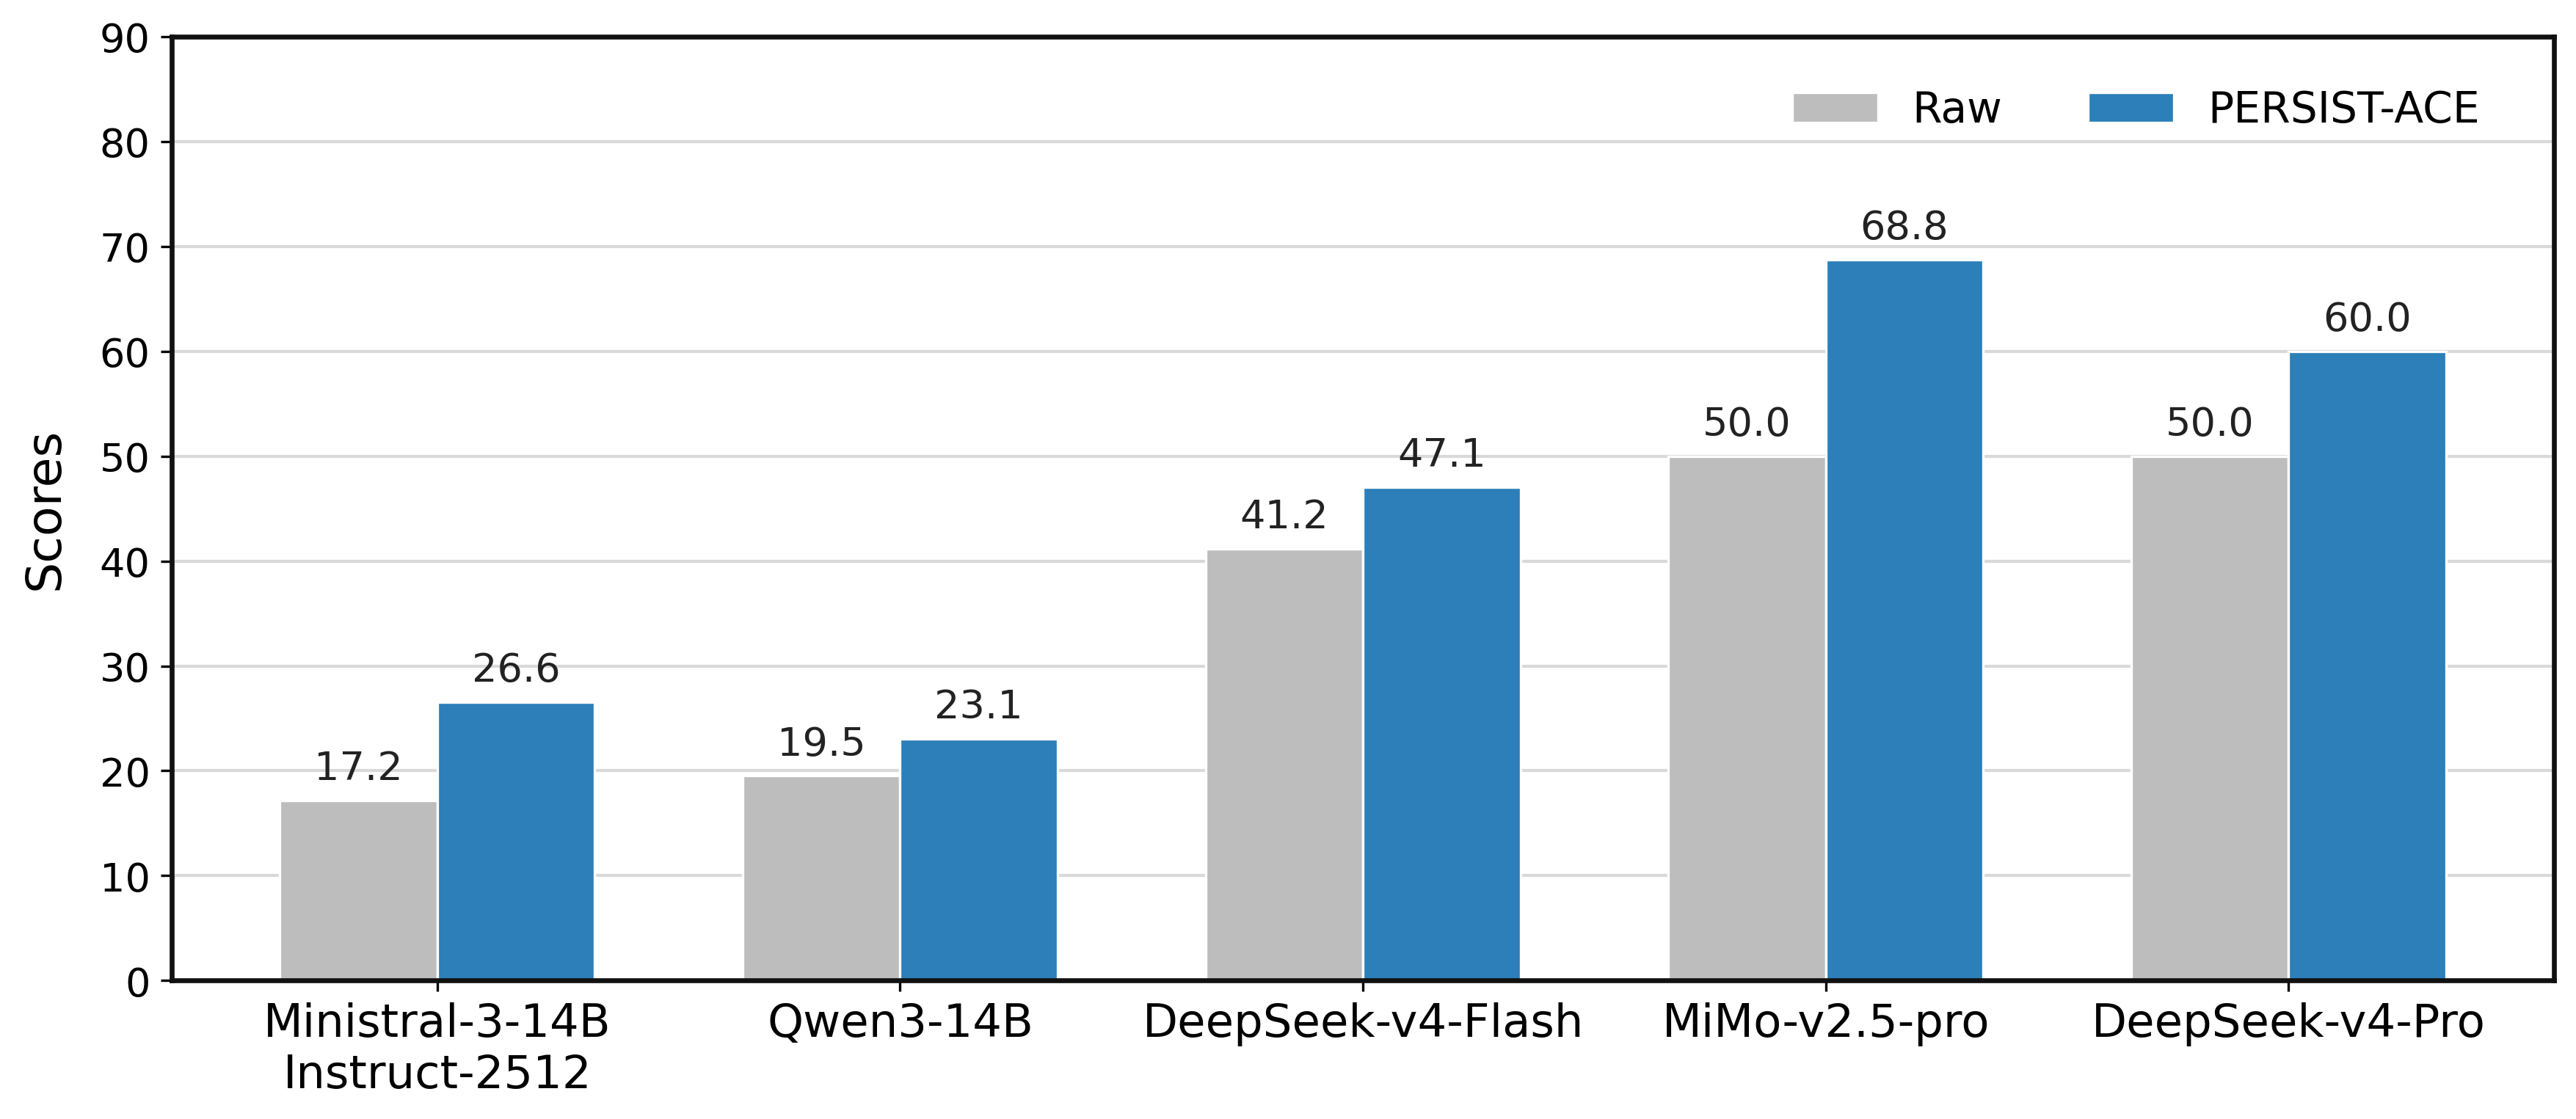
\includegraphics[width=\columnwidth]{figures/fig_statebench_fl_subset_scores.png}
\caption{STATE-Bench scores on task-runs whose Raw trajectory contains a
Functional Loop before intervention. PERSIST-ACE raises the score for all five
base models.}
\label{fig:functional-loop-subset-scores}
\end{figure}

\begin{figure}[!t]
\centering
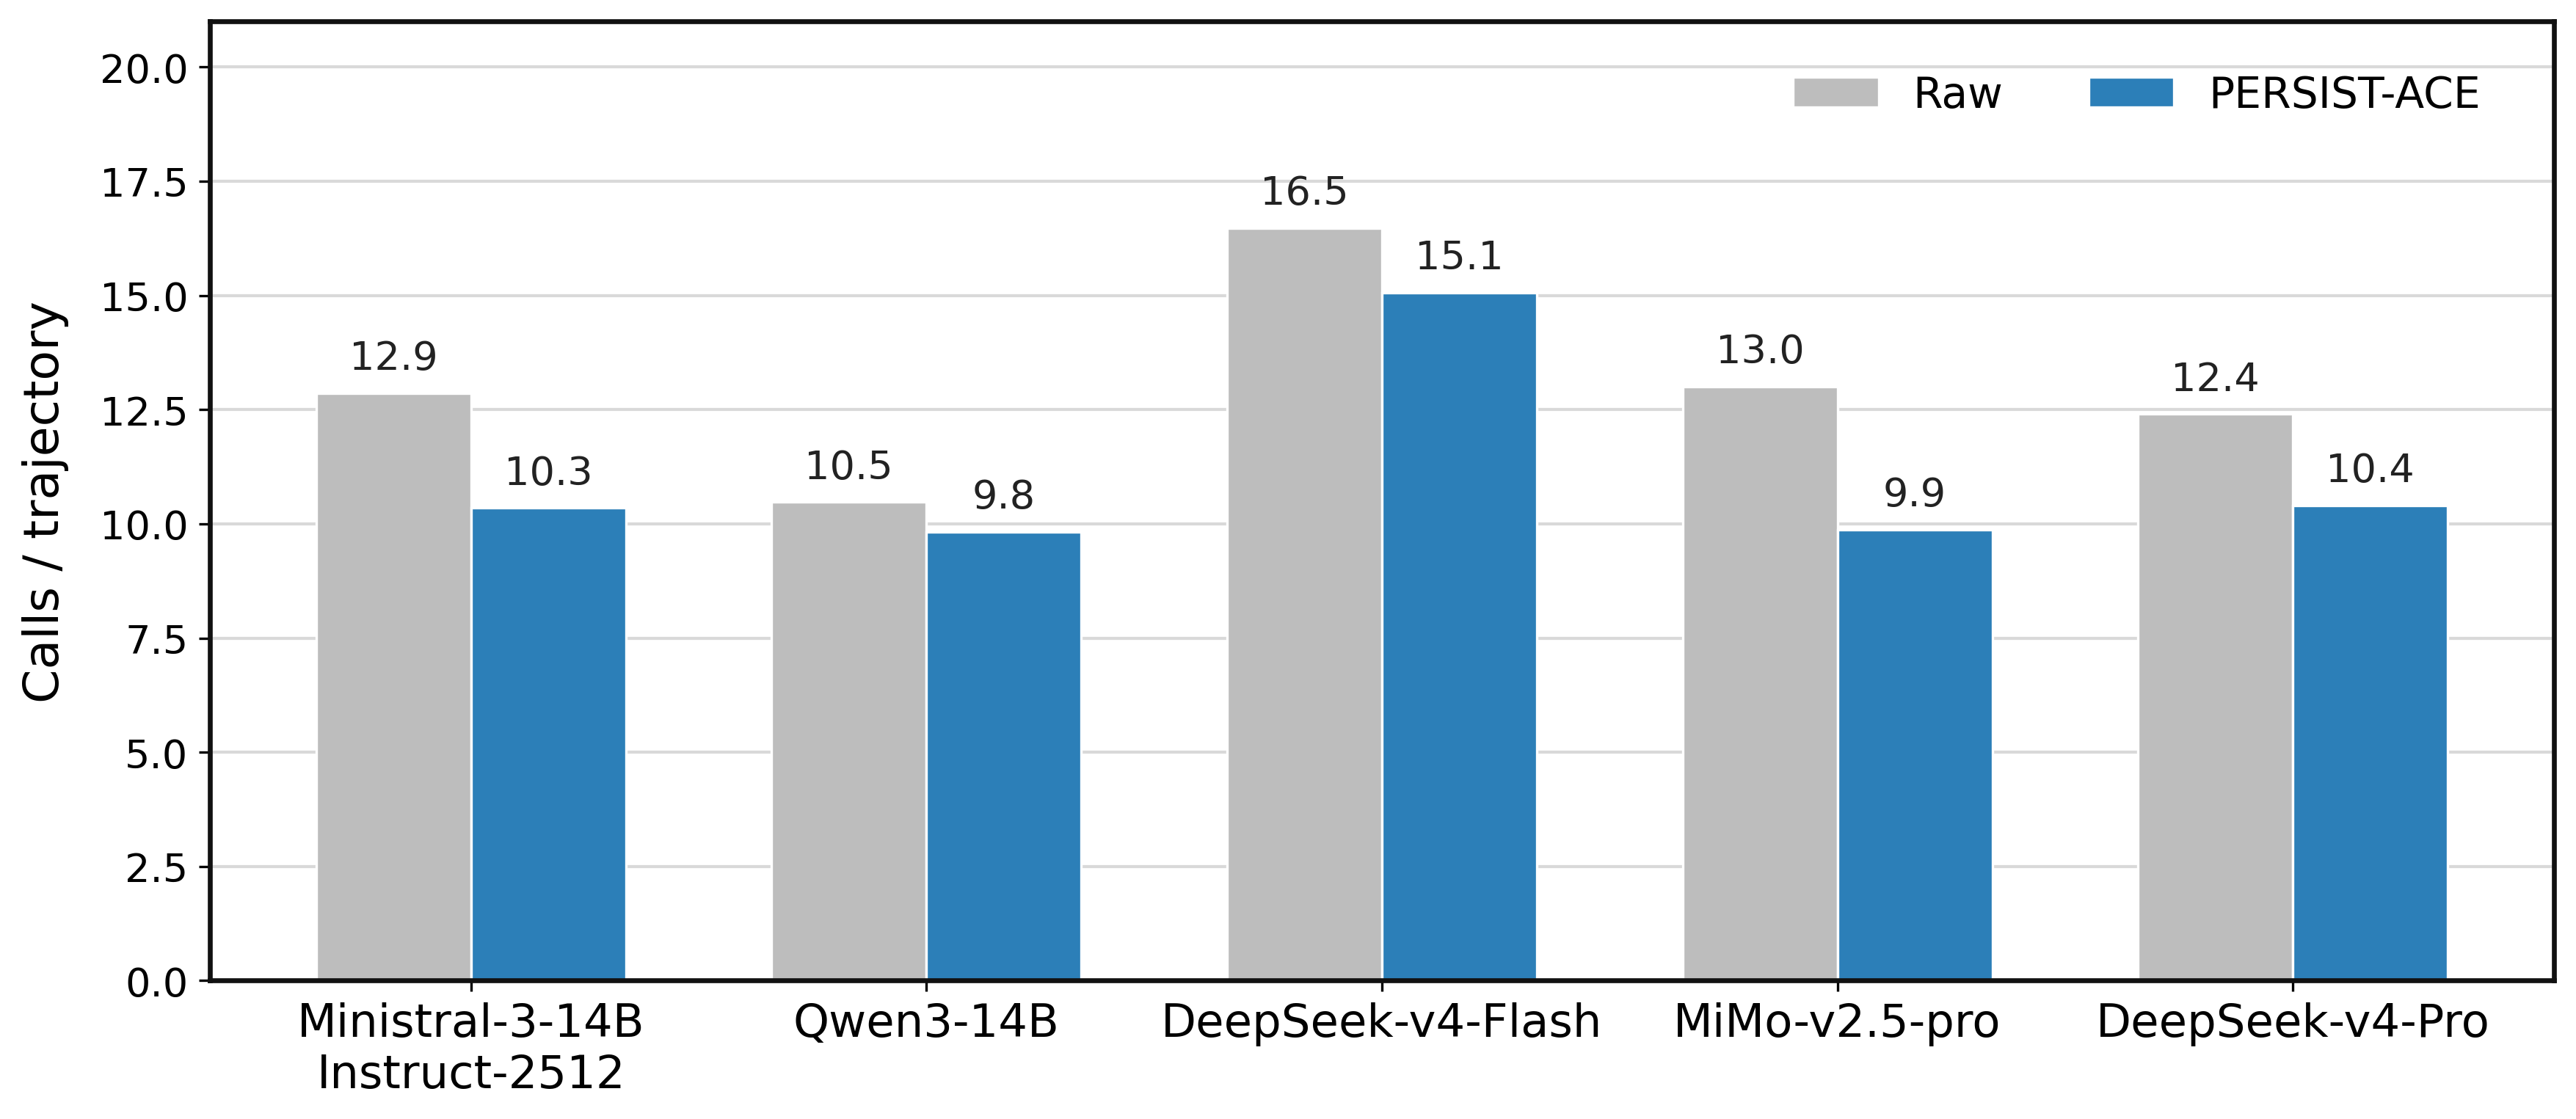
\includegraphics[width=\columnwidth]{figures/fig_statebench_fl_subset_calls.png}
\caption{Tool calls on the same Functional Loop-exposed task-runs used in
Figure~\ref{fig:functional-loop-subset-scores}. PERSIST-ACE reduces mean calls
for every base model.}
\label{fig:functional-loop-subset-calls}
\end{figure}

\textbf{Functional Loop-exposed trajectories.}
Figures~\ref{fig:functional-loop-subset-scores} and
\ref{fig:functional-loop-subset-calls} examine the subset that contained a
Functional Loop before intervention. Scores rise for all five models,
including lower- and higher-performing baselines, while tool calls fall in every
case. The largest score gains appear for MiMo-v2.5-Pro and DeepSeek-v4-Pro,
whereas even the smaller gains are accompanied by shorter trajectories. The
improvement is therefore not obtained by simply extending stalled runs. On the
subset identified by Functional Loops, PERSIST-ACE consistently reaches better
outcomes with less interaction, supporting the combination of Functional Loop
detection and grounded Card execution.

These subset results describe deployment behavior rather than an
action-level causal effect. The same-state experiment in
Table~\ref{tab:card-structure-ablation} provides the controlled evidence for
the recovery program itself.

\FloatBarrier
